% ES started writing and thinking sometime in		March 2011
% ES re-started writing 				2011-11-03
% after being interupted by job applications,
% childbirth, moving to Dresden, real plumbing, etc.

% For chaos:
\documentclass[aip,cha,showpacs,twocolumn, 
 		  reprint]{revtex4-1} % superscriptaddress, unsortedaddress



\usepackage{amsmath,amsfonts,amssymb,amsbsy,amscd}
\usepackage[usenames,dvipsnames]{color}
\usepackage{hyperref}
\usepackage{graphicx}
\usepackage{ifthen}

%%%%%%%%% Macros
%% ES: Please only add macros that will allow to easilly change journal.
%% Do not add macros to keep terminology, notation etc flexible. 
%% Internal edits/comments macros are OK, as are some math macros already added.


\newcommand{\beq}{\begin{equation}}
\newcommand{\eeq}{\end{equation}}
\newcommand{\bseq}{\begin{subequations}}
\newcommand{\eseq}{\end{subequations}}
\newcommand{\barr}{\begin{array}}
\newcommand{\earr}{\end{array}}

\newcommand{\rf}     [1] {~\cite{#1}}
\newcommand{\refref} [1] {Ref.~\cite{#1}}
\newcommand{\refrefs}[1] {Refs.~\cite{#1}}
\newcommand{\refeq}  [1] {(\ref{#1})}
\newcommand{\refeqs} [2]{(\ref{#1}--\ref{#2})}
\newcommand{\reffig} [1] {Fig.~\ref{#1}}
\newcommand{\refFig} [1] {Figure~\ref{#1}}
\newcommand{\refsect}[1] {Sect.~\ref{#1}}
\newcommand{\refappe}[1] {Appendix~\ref{#1}}
\newcommand{\reftab} [1] {table~\ref{#1}}

\newcommand{\etc}{{etc.}}       
\newcommand{\etal}{{\em et al.}}
\newcommand{\ie}{{i.e.}}        
\newcommand{\cf}{{\em cf.\ }}   
\newcommand{\eg}{{e.g.\ }}      

\newcommand{\KS}{Kuramoto-Siva\-shin\-sky}
\newcommand{\KSe}{Kuramoto-Siva\-shin\-sky equation} 
\newcommand{\pCf}{plane Couette flow}
\newcommand{\PCf}{Plane Couette flow}

\newcommand{\Rls}[1]{\ensuremath{\mathbb{R}^{#1}}}
\newcommand{\Clx}[1]{\ensuremath{\mathbb{C}^{#1}}}
\newcommand{\Un}[1]{\ensuremath{\textrm{U}(#1)}}         % in DasBuch
\newcommand{\On}[1]{\ensuremath{\textrm{O}(#1)}}
\newcommand{\SOn}[1]{\ensuremath{\textrm{SO}(#1)}}         % in DasBuch
\newcommand{\Dn}[1]{\ensuremath{\textrm{D}_{#1}}}              % in DasBuch
\newcommand{\Zn}[1]{\ensuremath{\textrm{C}_{#1}}}              % in DasBuch
\newcommand{\Ztwo}{\ensuremath{\textrm{C}_2}}                % in DasBuch
\newcommand{\Refl}{\ensuremath{\sigma}}    

\newcommand{\chebT}{\mathrm{T}}
\newcommand{\chebU}{\mathrm{U}}

\newcommand{\Nd}{\ensuremath{d}} % state-space dimension
\newcommand{\Nc}{\ensuremath{N}} % complex state-space dimension

\newcommand{\ii}{\ensuremath{\mathrm{i}}} % \sqrt{-1}

%%%%%%% From chaosbook def.tex (copy them if absolutely necessary)
\newcommand{\wwwcb}[1]{       % keep homepage flexible:
                  {\tt \href{http://ChaosBook.org#1}
              {ChaosBook.org#1}}}
\newcommand{\arXiv}[1]{
              {\tt \href{http://arXiv.org/abs/#1}{\goodbreak arXiv:#1}}}
\newcommand{\weblink}[1]{{\tt \href{http://#1}{#1}}}

%%%%%%% Setup hyperlinks
\definecolor{hreflinkcolor}{rgb}{0.13,0.17,0.83}
\hypersetup{colorlinks=true,urlcolor=hreflinkcolor,
		linkcolor=hreflinkcolor,citecolor=hreflinkcolor}
% Graphics files are in the figures/ directory
\graphicspath{{../../figs/}}
\bibliographystyle{apsrev4-1}


\begin{document}

% ES: Please permute names as appropriate.

\author{Evangelos Siminos} 
\email{siminos@gatech.edu}
\affiliation{School of Physics, 
	      Georgia Institute of Technology, Atlanta, GA 30332, USA}
\affiliation{Max Planck Institute for the Physics of Complex Systems, 
N\"othnitzer Stra\ss e 38, 01187 Dresden, Germany}

\author{Predrag Cvitanovi\'c}
\affiliation{School of Physics, 
	      Georgia Institute of Technology, Atlanta, GA 30332, USA}

\author{Ruslan L. Davidchack}
\affiliation{Department of Mathematics, 
	      University of Leicester, Leicester, LE1 7RH, UK}

\title{Freezing of all waves: global symmetry reduction in Kuramoto-Sivashinsky equation}

\date{\today}


%%%%%%%%%%%%%%%%%%%%%%%%%%%%%%%%%%%%%%%%%%%%%%%%%%%%%%%%%%%%%%%%%%%%%%%%%%%%%%%%
\begin{abstract}

\end{abstract}
%%%%%%%%%%%%%%%%%%%%%%%%%%%%%%%%%%%%%%%%%%%%%%%%%%%%%%%%%%%%%%%%%%%%%%%%%%%%%%%%

\pacs{}

\maketitle

%%%%%%%%%%%%%%%%%%%%%%%%%%%%%%%%%%%%%%%%%%%%%%%%%%%%%%%%%%%%%%%%%%%%%%%%%%%%%%%%

% \begin{quotation}
%  Leading paragraph
% \end{quotation}
% 

\section{Introduction\label{s:intro}}

% Recent developments in the study of fluids and other dissipative, 
% spatially-extended systems sugest that certain types of intrinsically 
% low-dimensional behaviour can be understood by means of the theory of
% dynamical systems. In particular, studies of the Kuramoto-Sivashinsky
% partial differential equation (PDE) and of the plane Couette flow indicate that
% the low-dimensional manifolds of unstable equilibria play the key role in
% organizing the high-dimensional state-space, in a way familiar from the study
% of low-dimensional systems of ordinary differential equations (ODEs). 
% An important limitation of studies that embrace this point of view is that,
% so far, the signifance of traveling wave solutions as organizing centers 
% has not been clarified, even though these constitute the most commonly 
% encountered stationary solutions in fluid flows.  
% 
% Wave motion appears as a result of the translational symmetry of the partial
% differential equations that describe continuous media, which in turn can be
% traced back to the basic assumptions on the nature of space and the physical
% laws. Waves which maintain a constant shape during their propagation, 
% also termed relative equilibria, are translationaly invariant solutions and can
% be thought of as equilibria in a comoving frame. However, we are interested here
% in a global state-space picture and, as multiple traveling waves of different
% speeds commonly exist for any given flow parameter, the use of a single
% co-moving frame is rendered problematic for our purposes. Moreover, solutions
% with broken symmetry also do exist, for instance modulated traveling waves in
% which the wave profile is characterized by a periodic modulation (whence the
% alternative name relative periodic orbit). Furthermore, the generic, 
% turbulent solutions are characterized by drifts along the direction of wave
% propagation. 
% 
% To illustrate how this obscures the understanding of global
% state-space geometry, we present in \reffig{f:ksIntro}(a) a state-space
% portrait of the Kuramoto-Sivashinsky (KS) flow 
% (introduced in \refsect{s:notions}), in a periodic spatial domain of length
% $L=22$. We think of the KS flow in terms of its $\Nd$-dimensional Fourier 
% space truncation, with $\Nd$ large enough for well-resolved simulations.   
% The projection in \reffig{f:ksIntro}(a) is onto the the real parts of
% the three leading Fourier modes and suffers from the tendency of solutions to drift 
% around (in Fourier space, translations become rotations). 
% 
% The main achievement of this paper is to show how the mess 
% of \reffig{f:ksIntro}(a) can be brought
% to the comprehensible and usefull representation of \reffig{f:ksIntro}(b) in
% which the role of unstable manifolds of traveling waves in organizing the global
% geometry becomes apparent. The means by which the transition from 
% \reffig{f:ksIntro}(a) to \reffig{f:ksIntro}(a) is achieved is \emph{symmetry
% reduction}: the variables onto which we project in \reffig{f:ksIntro}(b) are
% translationaly invariant (or rotationally invariant if we think in terms of
% Fourier modes) and span the $\Nd-1$-dimensional \emph{reduced space} in which
% wave motion appears frozen.
% 

\section{Basic notions\label{s:notions}}

\section{From moving frames to invariant variables}

We begin by computing invariants for the ``standard action''
of $\SOn{2}$ on $\Clx{N}\cong\Rls{2N}$
which we write here as
% \beq
% 	\left(\barr{cc} \overline{b}_k \\ \overline{c}_k\earr \right)=\left(\barr{cc}
% 			    			\cos(k\theta) & -\sin(k\theta)\\
% 						\sin(k\theta) & \cos(k\theta)\\
% 			   			\earr	
% 						\right) \left(\barr{cc} b_k \\ c_k\earr\right)\,,\ \ k=1,\ldots N\,.
% 	\label{eq:SO2stand}
% \eeq
\bseq\label{eq:SO2stand}
  \begin{align}
	  \overline{b}_k &= \cos(k\theta)\,b_k - \sin(k\theta)\,c_k\,\label{eq:SO2stand1}\\
	  \overline{c}_k &= \sin(k\theta)\,b_k + \cos(k\theta)\,c_k\,,\label{eq:SO2stand2}
  \end{align}
\eseq
with $a_k=b_k+i c_k\,,\ b_k,c_k\in\Rls{}$ and $k=1,\ldots N$.
The choice of a slice is arbitrary; here we choose
\beq
 	\overline{c}_1=0\,,\qquad \overline{b}_1>0\,
\eeq
which leads to
\beq
	\overline{c}_1 = b_1\,\sin\theta + c_1\,\cos\theta  = 0\,
	\label{eq:SO2norm}
\eeq
and the ``moving frame''
\beq
	\theta=-\tan^{-1}\frac{c_1}{b_1}\,.
	\label{eq:SO2mf}
\eeq
Here $\tan^{-1}$ distinguishes quadrants, so that our choice of a slice
results to 
\beq\label{eq:phi1}
  \theta=-\phi_1\,,
\eeq
where $\phi_1$ the polar angle in the $a_1$ Fourier
subspace. Pluging \refeq{eq:phi1} into
transformations \refeq{eq:SO2stand} we get:
\bseq\label{eq:SO2cheb}
  \begin{align}
    \overline{b}_k &= 
		    b_k\, \chebT_k\left(b_1/r_1\right)+
		    c_k\,\frac{c_1}{r_1} \chebU_{k-1}\left(b_1/r_1\right)\,, \label{eq:SO2cheb1}\\
    \overline{c}_k &=
		    b_k\, \frac{c_1}{r_1} \chebU_{k-1}\left(b_1/r_1\right)+
		    c_k\,\chebT_k\left(b_1/r_1\right)\,,  \label{eq:SO2cheb2}
  \end{align}
\eseq
for $k=1,\ldots N$, where $r_k\equiv\sqrt{b_i^2+c_i^2}$ and $\chebT_k,\,\chebU_k$
are Chebyshev polynomials of the first and second type, respectively. 
Note that for $k=1$ we get $\overline{b}_1=r_1,\, \overline{c}_1=0$. 
Thus we have arrived at a system of $2N-1$ variables, which according to 
theorems of Fels and Olver\rf{FelsOlver98,FelsOlver99} are
$\SOn{2}$-invariant and functionally independent. They therefore serve the goal
of unique identification of group orbits, at least in the neighborhood of the
slice. Under reflections $\Refl a_k \mapsto-b_k+\ii c_k$ we see that
\bseq\label{eq:SO2chebRefl}
 \begin{align}
  \overline{b}_k \mapsto (-1)^{k+1}\, \overline{b}_k\,,\\ 
  \overline{c}_k \mapsto (-1)^{k}\, \overline{c}_k\,.
 \end{align}
\eseq
 To factor out the discrete reflection symmetry in \refeq{eq:SO2chebRefl} we can
introduce a fundamental domain by taking the absolute value of those variables
which are equivariant under $\Refl$, so that we are led to
\bseq\label{eq:O2cheb}
  \begin{align}
    \overline{b}'_k &= 
		    |\overline{b}_k|\,, \\
    \overline{c}'_k &=
		    \overline{c}_k\,.
  \end{align}
for $k$ even, and
  \begin{align}
    \overline{b}'_k &= 
		    \overline{b}_k\,, \\
    \overline{c}'_k &=
		    |\overline{c}_k|\,.
  \end{align}
for $k$ odd.
\eseq

However, invariant variables \refeq{eq:O2cheb} can be seen to be singular as 
$r_1\rightarrow1$. The relation of such singularities to the choice of a slice
has been discussed in \refrefs{SiminosThesis, SiCvi10, FrCv11}. In 
\refrefs{SiCvi10, FrCv11}, and also in \refref{rowley_reconstruction_2000},
the use of multiple local slices to cover state-space has been proposed.
However, the tasks of picking such a set of slices 
and piecing them together in a manner that does not obscure the global picture
are highly non-trivial when one works in high-dimensional spaces and we know
of no successful implementation of the tesselation idea set forth in 
\refref{FrCv11}. Here we will take a different path and motivate some 
modifications of equations \refeq{eq:O2cheb} until we obtain 
\emph{globally} well behaved transformations to invariant variables.

To shed more light into the origin of the singularities in \refeq{eq:O2cheb}, 
we use the identity 
$\alpha\cos(\phi)+\beta\sin(\phi)=\sqrt{\alpha^2+\beta^2}\cos(x-\tan^{-1}(\beta/\alpha))$
and plug \refeq{eq:phi1} into \refeq{eq:SO2stand}, to arrive to the
``polar'' form of \refeq{eq:SO2cheb}
\bseq\label{eq:SO2polar}
  \begin{align}
    \overline{b}_k &= 
		    r_k\, \cos(\phi_k-k\,\phi_1)\,, \label{eq:SO2polar1}\\
    \overline{c}_k &=
		    r_k\, \sin(\phi_k-k\,\phi_1)\,,\label{eq:SO2polar2}
  \end{align}
\eseq
where $\phi_k$ the polar angle in the $a_k$ Fourier subspace. In this coupled-polar
representation, it becomes apparent that the singularities of \refeq{eq:SO2cheb}
are related to the familiar singularities of polar variables at the origin.
Tuckerman\rf{tuckerman89} showed that terms of the form $\psi_{nk}(r,\phi)=r^n\exp(\ii\, k\,\phi)$ 
which appear in cylindrical coordinate $(r,\phi,z)$ discretizations of PDEs 
are typically non-smooth at the origin. The problem is traced to rapid 
oscillations of $\psi_{nk}$ (with $\phi$) as $r\rightarrow0$ and Tuckerman\rf{tuckerman89} shows
that such oscillations are heavily damped near the origin for
$\psi_{nk}$ with $n\geq k$. The prescription put forth by Tuckerman\rf{tuckerman89} to 
construct a smooth basis for the numerical discretization of
PDEs is to keep only terms with $n\geq k$ 
(with some additional technical conditions).

The simplest way to modify variables \refeq{eq:SO2polar} to fullfil Tuckerman's
criterion is to multiply the right hand side by $r_1^k$. This would lead us to 
work with invariant polynomials of order $k+1$ for the $k$'th Fourier subspace, 
as seen from \refeq{eq:SO2cheb}, resulting in highly deformed $a_k$ components
(and numerical underflow problems). Since our main goal is to investigate the
topology of the attractor we can instead aim at merely continuous transformations.
Note also, that the introduction of a fundamental domain for discrete symmetry
reduction destroys smoothness of the transformations, even if it is initially
imposed in continuous symmetry reduction.
Thus, we simply multiply the right-hand side of \refeq{eq:SO2polar} with $r_1$,
so that our modified set of $SO(2)$-invariants reads
\bseq\label{eq:SO2polarCont}
  \begin{align}
    \tilde{b}_k &= 
		    r_1\,\overline{b}_k\,, \label{eq:SO2polarCont1}\\
    \tilde{c}_k &=
		    r_1\,\overline{c}_k\,.\label{eq:SO2polarCont2}
  \end{align}
\eseq

Transformations \refeq{eq:SO2polarCont}, although continuous at
$r_1=0$ fail to distinguish points in the $a_k$ Fourier subspace when $r_1=0$.
This a rather serious limitation, since non-trivial $N$-cell equilibria of
KSe are mapped to the origin under \refeq{eq:SO2polarCont}.
We can bypass this difficulty by adding an $r_k^2$ factor into the variables
associated with the $k$'th Fourier subspace, in such a way that it respects
reflection equivariance as expressed by \refeq{eq:SO2chebRefl}, to arrive to
\bseq\label{eq:SO2inv}
  \begin{align}
    \tilde{b}'_k &= 
		    r_1\,r_k\, \cos(\phi_k-k\,\phi_1)\,, \\
    \tilde{c}'_k &=
		    r_k^2+r_1\,r_k\,\sin(\phi_k-k\,\phi_1)\,,
  \end{align}
for $k$ even, and
  \begin{align}
    \tilde{b}'_k &= 
		    r_k^2+r_1\,r_k\, \cos(\phi_k-k\,\phi_1)\,, \\
    \tilde{c}'_k &=
		    r_1\,r_k\, \cos(\phi_k-k\,\phi_1)\,,
  \end{align}
for $k$ odd.
\eseq
% \bseq\label{eq:SO2polarContInd}
%   \begin{align}
%     \tilde{b}_k &= 
% 		    \frac{1}{2}(1-(-1)^k)\,r_k^2+r_1\,\overline{b}_k\,, \label{eq:SO2polarCont1}\\
%     \tilde{c}_k &=
% 		    \frac{1}{2}(1-(-1)^{k+1})\,\,r_k^2+r_1\,\overline{c}_k\,.\label{eq:SO2polarCont2}
%   \end{align}
% \eseq

% Finally we need to factor out the discrete reflectional symmetry still present 
% in \refeq{eq:SO2inv}. A simple but effective way to achieve this is
% by taking the absolute value of $\Refl$-equivariant variables 
% in \refeq{eq:SO2inv}. 
As before, we factor out reflection symmetry by taking the absolute value 
of $\Refl$-equivariant variables in \refeq{eq:SO2inv}. 
Thus we are led to $\On{2}$-invariant variables
\bseq\label{eq:O2inv}
  \begin{align}
    \beta_k &= 
		    r_1\,r_k\, |\cos(\phi_k-k\,\phi_1)|\,, \\
    \gamma_k &=
		    r_k^2+r_1\,r_k\,\sin(\phi_k-k\,\phi_1)\,,
  \end{align}
for $k$ even, and
  \begin{align}
    \beta_k &= 
		    r_k^2+r_1\,r_k\, \cos(\phi_k-k\,\phi_1)\,, \\
    \gamma_k &=
		    r_1\,r_k\, |\cos(\phi_k-k\,\phi_1)|\,,
  \end{align}
for $k$ odd.
\eseq
 
\section{KS reduced state-space} 

\begin{figure}
% ES used siminos/chao/matlab/ruslan/ks22rpoCompInv.m
 (a)~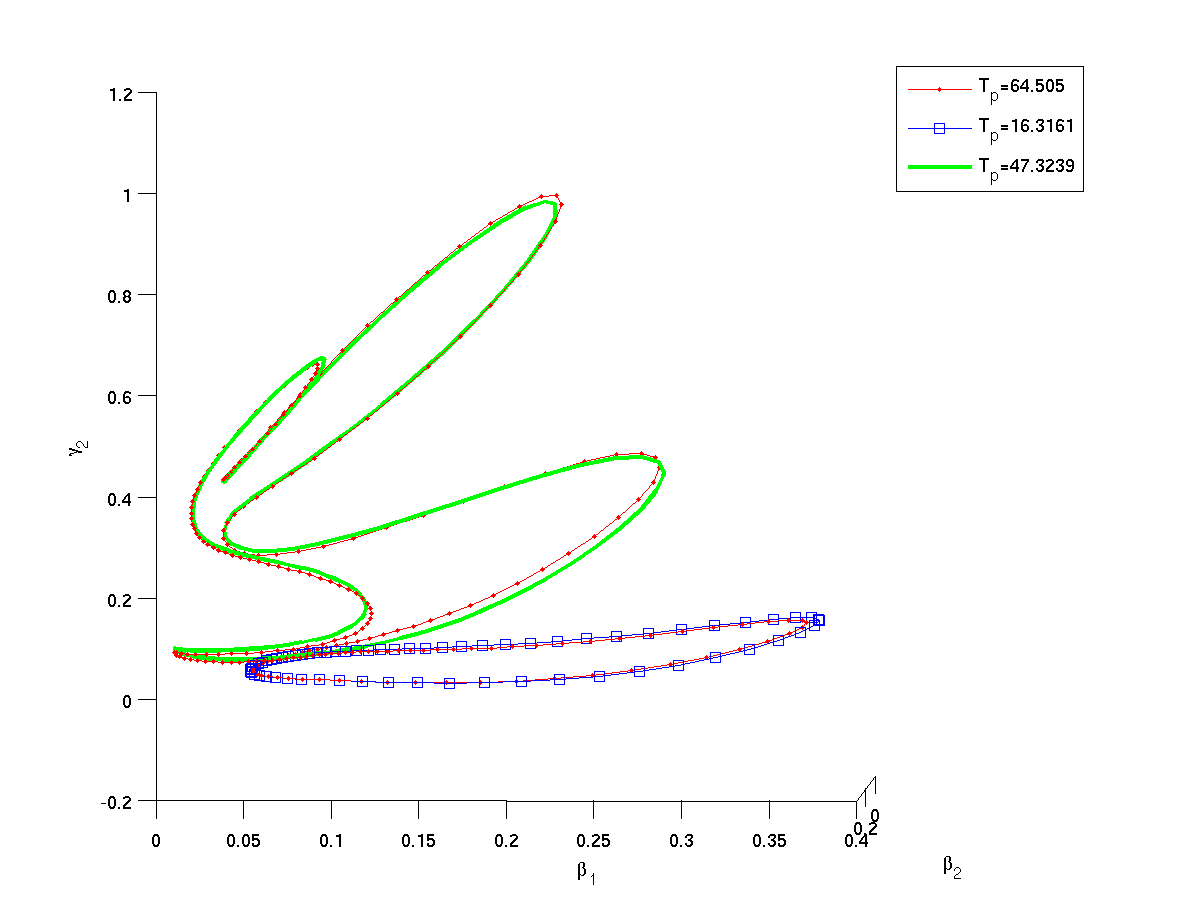
\includegraphics[width=0.40\textwidth]{../figs/ks22rpo_shad1}
 (b)~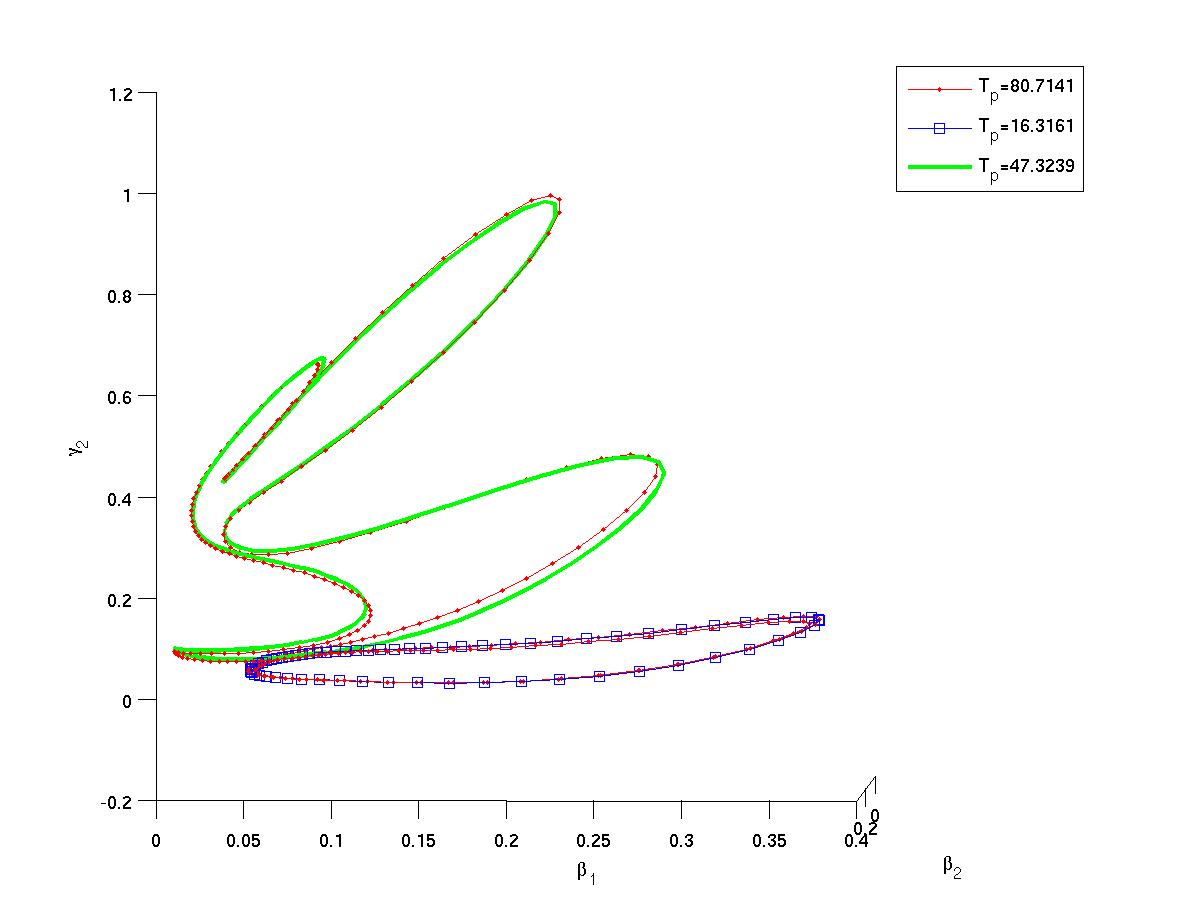
\includegraphics[width=0.40\textwidth]{../figs/ks22rpo_shad2}
\caption{
 Shadowing of relative periodic orbits of \KSe\ for $L=22.0$ (see \refref{SCD07}), 
projected in $\beta_1, \beta_2, \gamma_2$ of 
\refeq{eq:O2inv}. (a) Orbit with period $T_{64.51}$ is shadowed by
orbits $T_{16.32}$ and $T_{47.32}$, (b) Orbit with period 
$T_{80.71}$ is shadowed by orbits $T_{16.32}$ and $T_{47.32}$. Note
that $T_{80.71}$ traces $T_{16.32}$ twice.
% ES: We can hope for some symbolic dynamics in which  $T_{64.51}$  is $01$ and
% $T_{80.71}$ is $001$.
}
\label{fig:rpo_shad}
\end{figure}


\section{Conclusions}

Motivating \refeq{eq:O2inv} is still rough around the edges, but the final result is
1) easilly seen to be $\On{2}$-invariant, 2) easilly and economically 
implemented numerically, requiring no computer algebra, 3) it scales well
with the dimension of phase space, 4) it is global requires no further
thinking of singularities and can thus be used in automated searches for
neigborhing orbits in sets of thousands orbits. This is how commencing with the 
organization of relative periodic orbits in families, as in \reffig{fig:rpo_shad},
became possible.

\bibliography{../bibtex/siminos}

\end{document}